
% Default to the notebook output style

    


% Inherit from the specified cell style.




    
\documentclass[11pt,french]{article}

    
    \usepackage{babel}
    \usepackage[T1]{fontenc}
    % Nicer default font (+ math font) than Computer Modern for most use cases
    \usepackage{mathpazo}

    % Basic figure setup, for now with no caption control since it's done
    % automatically by Pandoc (which extracts ![](path) syntax from Markdown).
    \usepackage{graphicx}
    % We will generate all images so they have a width \maxwidth. This means
    % that they will get their normal width if they fit onto the page, but
    % are scaled down if they would overflow the margins.
    \makeatletter
    \def\maxwidth{\ifdim\Gin@nat@width>\linewidth\linewidth
    \else\Gin@nat@width\fi}
    \makeatother
    \let\Oldincludegraphics\includegraphics
    % Set max figure width to be 80% of text width, for now hardcoded.
    \renewcommand{\includegraphics}[1]{\Oldincludegraphics[width=.8\maxwidth]{#1}}
    % Ensure that by default, figures have no caption (until we provide a
    % proper Figure object with a Caption API and a way to capture that
    % in the conversion process - todo).
    \usepackage{caption}
    \DeclareCaptionLabelFormat{nolabel}{}
    \captionsetup{labelformat=nolabel}

    \usepackage{adjustbox} % Used to constrain images to a maximum size 
    \usepackage{xcolor} % Allow colors to be defined
    \usepackage{enumerate} % Needed for markdown enumerations to work
    \usepackage{geometry} % Used to adjust the document margins
    \usepackage{amsmath} % Equations
    \usepackage{amssymb} % Equations
    \usepackage{textcomp} % defines textquotesingle
    % Hack from http://tex.stackexchange.com/a/47451/13684:
    \AtBeginDocument{%
        \def\PYZsq{\textquotesingle}% Upright quotes in Pygmentized code
    }
    \usepackage{upquote} % Upright quotes for verbatim code
    \usepackage{eurosym} % defines \euro
    \usepackage[mathletters]{ucs} % Extended unicode (utf-8) support
    \usepackage[utf8x]{inputenc} % Allow utf-8 characters in the tex document
    \usepackage{fancyvrb} % verbatim replacement that allows latex
    \usepackage{grffile} % extends the file name processing of package graphics 
                         % to support a larger range 
    % The hyperref package gives us a pdf with properly built
    % internal navigation ('pdf bookmarks' for the table of contents,
    % internal cross-reference links, web links for URLs, etc.)
    \usepackage{hyperref}
    \usepackage{longtable} % longtable support required by pandoc >1.10
    \usepackage{booktabs}  % table support for pandoc > 1.12.2
    \usepackage[inline]{enumitem} % IRkernel/repr support (it uses the enumerate* environment)
    \usepackage[normalem]{ulem} % ulem is needed to support strikethroughs (\sout)
                                % normalem makes italics be italics, not underlines
    \usepackage{mathrsfs}
    

    
    
    % Colors for the hyperref package
    \definecolor{urlcolor}{rgb}{0,.145,.698}
    \definecolor{linkcolor}{rgb}{.71,0.21,0.01}
    \definecolor{citecolor}{rgb}{.12,.54,.11}

    % ANSI colors
    \definecolor{ansi-black}{HTML}{3E424D}
    \definecolor{ansi-black-intense}{HTML}{282C36}
    \definecolor{ansi-red}{HTML}{E75C58}
    \definecolor{ansi-red-intense}{HTML}{B22B31}
    \definecolor{ansi-green}{HTML}{00A250}
    \definecolor{ansi-green-intense}{HTML}{007427}
    \definecolor{ansi-yellow}{HTML}{DDB62B}
    \definecolor{ansi-yellow-intense}{HTML}{B27D12}
    \definecolor{ansi-blue}{HTML}{208FFB}
    \definecolor{ansi-blue-intense}{HTML}{0065CA}
    \definecolor{ansi-magenta}{HTML}{D160C4}
    \definecolor{ansi-magenta-intense}{HTML}{A03196}
    \definecolor{ansi-cyan}{HTML}{60C6C8}
    \definecolor{ansi-cyan-intense}{HTML}{258F8F}
    \definecolor{ansi-white}{HTML}{C5C1B4}
    \definecolor{ansi-white-intense}{HTML}{A1A6B2}
    \definecolor{ansi-default-inverse-fg}{HTML}{FFFFFF}
    \definecolor{ansi-default-inverse-bg}{HTML}{000000}

    % commands and environments needed by pandoc snippets
    % extracted from the output of `pandoc -s`
    \providecommand{\tightlist}{%
      \setlength{\itemsep}{0pt}\setlength{\parskip}{0pt}}
    \DefineVerbatimEnvironment{Highlighting}{Verbatim}{commandchars=\\\{\}}
    % Add ',fontsize=\small' for more characters per line
    \newenvironment{Shaded}{}{}
    \newcommand{\KeywordTok}[1]{\textcolor[rgb]{0.00,0.44,0.13}{\textbf{{#1}}}}
    \newcommand{\DataTypeTok}[1]{\textcolor[rgb]{0.56,0.13,0.00}{{#1}}}
    \newcommand{\DecValTok}[1]{\textcolor[rgb]{0.25,0.63,0.44}{{#1}}}
    \newcommand{\BaseNTok}[1]{\textcolor[rgb]{0.25,0.63,0.44}{{#1}}}
    \newcommand{\FloatTok}[1]{\textcolor[rgb]{0.25,0.63,0.44}{{#1}}}
    \newcommand{\CharTok}[1]{\textcolor[rgb]{0.25,0.44,0.63}{{#1}}}
    \newcommand{\StringTok}[1]{\textcolor[rgb]{0.25,0.44,0.63}{{#1}}}
    \newcommand{\CommentTok}[1]{\textcolor[rgb]{0.38,0.63,0.69}{\textit{{#1}}}}
    \newcommand{\OtherTok}[1]{\textcolor[rgb]{0.00,0.44,0.13}{{#1}}}
    \newcommand{\AlertTok}[1]{\textcolor[rgb]{1.00,0.00,0.00}{\textbf{{#1}}}}
    \newcommand{\FunctionTok}[1]{\textcolor[rgb]{0.02,0.16,0.49}{{#1}}}
    \newcommand{\RegionMarkerTok}[1]{{#1}}
    \newcommand{\ErrorTok}[1]{\textcolor[rgb]{1.00,0.00,0.00}{\textbf{{#1}}}}
    \newcommand{\NormalTok}[1]{{#1}}
    
    % Additional commands for more recent versions of Pandoc
    \newcommand{\ConstantTok}[1]{\textcolor[rgb]{0.53,0.00,0.00}{{#1}}}
    \newcommand{\SpecialCharTok}[1]{\textcolor[rgb]{0.25,0.44,0.63}{{#1}}}
    \newcommand{\VerbatimStringTok}[1]{\textcolor[rgb]{0.25,0.44,0.63}{{#1}}}
    \newcommand{\SpecialStringTok}[1]{\textcolor[rgb]{0.73,0.40,0.53}{{#1}}}
    \newcommand{\ImportTok}[1]{{#1}}
    \newcommand{\DocumentationTok}[1]{\textcolor[rgb]{0.73,0.13,0.13}{\textit{{#1}}}}
    \newcommand{\AnnotationTok}[1]{\textcolor[rgb]{0.38,0.63,0.69}{\textbf{\textit{{#1}}}}}
    \newcommand{\CommentVarTok}[1]{\textcolor[rgb]{0.38,0.63,0.69}{\textbf{\textit{{#1}}}}}
    \newcommand{\VariableTok}[1]{\textcolor[rgb]{0.10,0.09,0.49}{{#1}}}
    \newcommand{\ControlFlowTok}[1]{\textcolor[rgb]{0.00,0.44,0.13}{\textbf{{#1}}}}
    \newcommand{\OperatorTok}[1]{\textcolor[rgb]{0.40,0.40,0.40}{{#1}}}
    \newcommand{\BuiltInTok}[1]{{#1}}
    \newcommand{\ExtensionTok}[1]{{#1}}
    \newcommand{\PreprocessorTok}[1]{\textcolor[rgb]{0.74,0.48,0.00}{{#1}}}
    \newcommand{\AttributeTok}[1]{\textcolor[rgb]{0.49,0.56,0.16}{{#1}}}
    \newcommand{\InformationTok}[1]{\textcolor[rgb]{0.38,0.63,0.69}{\textbf{\textit{{#1}}}}}
    \newcommand{\WarningTok}[1]{\textcolor[rgb]{0.38,0.63,0.69}{\textbf{\textit{{#1}}}}}
    
    
    % Define a nice break command that doesn't care if a line doesn't already
    % exist.
    \def\br{\hspace*{\fill} \\* }
    % Math Jax compatibility definitions
    \def\gt{>}
    \def\lt{<}
    \let\Oldtex\TeX
    \let\Oldlatex\LaTeX
    \renewcommand{\TeX}{\textrm{\Oldtex}}
    \renewcommand{\LaTeX}{\textrm{\Oldlatex}}
    % Document parameters
    % Document title
    \title{Chap. II Les fonctions}
    
    
    
    
    

    % Pygments definitions
    
\makeatletter
\def\PY@reset{\let\PY@it=\relax \let\PY@bf=\relax%
    \let\PY@ul=\relax \let\PY@tc=\relax%
    \let\PY@bc=\relax \let\PY@ff=\relax}
\def\PY@tok#1{\csname PY@tok@#1\endcsname}
\def\PY@toks#1+{\ifx\relax#1\empty\else%
    \PY@tok{#1}\expandafter\PY@toks\fi}
\def\PY@do#1{\PY@bc{\PY@tc{\PY@ul{%
    \PY@it{\PY@bf{\PY@ff{#1}}}}}}}
\def\PY#1#2{\PY@reset\PY@toks#1+\relax+\PY@do{#2}}

\expandafter\def\csname PY@tok@w\endcsname{\def\PY@tc##1{\textcolor[rgb]{0.73,0.73,0.73}{##1}}}
\expandafter\def\csname PY@tok@c\endcsname{\let\PY@it=\textit\def\PY@tc##1{\textcolor[rgb]{0.25,0.50,0.50}{##1}}}
\expandafter\def\csname PY@tok@cp\endcsname{\def\PY@tc##1{\textcolor[rgb]{0.74,0.48,0.00}{##1}}}
\expandafter\def\csname PY@tok@k\endcsname{\let\PY@bf=\textbf\def\PY@tc##1{\textcolor[rgb]{0.00,0.50,0.00}{##1}}}
\expandafter\def\csname PY@tok@kp\endcsname{\def\PY@tc##1{\textcolor[rgb]{0.00,0.50,0.00}{##1}}}
\expandafter\def\csname PY@tok@kt\endcsname{\def\PY@tc##1{\textcolor[rgb]{0.69,0.00,0.25}{##1}}}
\expandafter\def\csname PY@tok@o\endcsname{\def\PY@tc##1{\textcolor[rgb]{0.40,0.40,0.40}{##1}}}
\expandafter\def\csname PY@tok@ow\endcsname{\let\PY@bf=\textbf\def\PY@tc##1{\textcolor[rgb]{0.67,0.13,1.00}{##1}}}
\expandafter\def\csname PY@tok@nb\endcsname{\def\PY@tc##1{\textcolor[rgb]{0.00,0.50,0.00}{##1}}}
\expandafter\def\csname PY@tok@nf\endcsname{\def\PY@tc##1{\textcolor[rgb]{0.00,0.00,1.00}{##1}}}
\expandafter\def\csname PY@tok@nc\endcsname{\let\PY@bf=\textbf\def\PY@tc##1{\textcolor[rgb]{0.00,0.00,1.00}{##1}}}
\expandafter\def\csname PY@tok@nn\endcsname{\let\PY@bf=\textbf\def\PY@tc##1{\textcolor[rgb]{0.00,0.00,1.00}{##1}}}
\expandafter\def\csname PY@tok@ne\endcsname{\let\PY@bf=\textbf\def\PY@tc##1{\textcolor[rgb]{0.82,0.25,0.23}{##1}}}
\expandafter\def\csname PY@tok@nv\endcsname{\def\PY@tc##1{\textcolor[rgb]{0.10,0.09,0.49}{##1}}}
\expandafter\def\csname PY@tok@no\endcsname{\def\PY@tc##1{\textcolor[rgb]{0.53,0.00,0.00}{##1}}}
\expandafter\def\csname PY@tok@nl\endcsname{\def\PY@tc##1{\textcolor[rgb]{0.63,0.63,0.00}{##1}}}
\expandafter\def\csname PY@tok@ni\endcsname{\let\PY@bf=\textbf\def\PY@tc##1{\textcolor[rgb]{0.60,0.60,0.60}{##1}}}
\expandafter\def\csname PY@tok@na\endcsname{\def\PY@tc##1{\textcolor[rgb]{0.49,0.56,0.16}{##1}}}
\expandafter\def\csname PY@tok@nt\endcsname{\let\PY@bf=\textbf\def\PY@tc##1{\textcolor[rgb]{0.00,0.50,0.00}{##1}}}
\expandafter\def\csname PY@tok@nd\endcsname{\def\PY@tc##1{\textcolor[rgb]{0.67,0.13,1.00}{##1}}}
\expandafter\def\csname PY@tok@s\endcsname{\def\PY@tc##1{\textcolor[rgb]{0.73,0.13,0.13}{##1}}}
\expandafter\def\csname PY@tok@sd\endcsname{\let\PY@it=\textit\def\PY@tc##1{\textcolor[rgb]{0.73,0.13,0.13}{##1}}}
\expandafter\def\csname PY@tok@si\endcsname{\let\PY@bf=\textbf\def\PY@tc##1{\textcolor[rgb]{0.73,0.40,0.53}{##1}}}
\expandafter\def\csname PY@tok@se\endcsname{\let\PY@bf=\textbf\def\PY@tc##1{\textcolor[rgb]{0.73,0.40,0.13}{##1}}}
\expandafter\def\csname PY@tok@sr\endcsname{\def\PY@tc##1{\textcolor[rgb]{0.73,0.40,0.53}{##1}}}
\expandafter\def\csname PY@tok@ss\endcsname{\def\PY@tc##1{\textcolor[rgb]{0.10,0.09,0.49}{##1}}}
\expandafter\def\csname PY@tok@sx\endcsname{\def\PY@tc##1{\textcolor[rgb]{0.00,0.50,0.00}{##1}}}
\expandafter\def\csname PY@tok@m\endcsname{\def\PY@tc##1{\textcolor[rgb]{0.40,0.40,0.40}{##1}}}
\expandafter\def\csname PY@tok@gh\endcsname{\let\PY@bf=\textbf\def\PY@tc##1{\textcolor[rgb]{0.00,0.00,0.50}{##1}}}
\expandafter\def\csname PY@tok@gu\endcsname{\let\PY@bf=\textbf\def\PY@tc##1{\textcolor[rgb]{0.50,0.00,0.50}{##1}}}
\expandafter\def\csname PY@tok@gd\endcsname{\def\PY@tc##1{\textcolor[rgb]{0.63,0.00,0.00}{##1}}}
\expandafter\def\csname PY@tok@gi\endcsname{\def\PY@tc##1{\textcolor[rgb]{0.00,0.63,0.00}{##1}}}
\expandafter\def\csname PY@tok@gr\endcsname{\def\PY@tc##1{\textcolor[rgb]{1.00,0.00,0.00}{##1}}}
\expandafter\def\csname PY@tok@ge\endcsname{\let\PY@it=\textit}
\expandafter\def\csname PY@tok@gs\endcsname{\let\PY@bf=\textbf}
\expandafter\def\csname PY@tok@gp\endcsname{\let\PY@bf=\textbf\def\PY@tc##1{\textcolor[rgb]{0.00,0.00,0.50}{##1}}}
\expandafter\def\csname PY@tok@go\endcsname{\def\PY@tc##1{\textcolor[rgb]{0.53,0.53,0.53}{##1}}}
\expandafter\def\csname PY@tok@gt\endcsname{\def\PY@tc##1{\textcolor[rgb]{0.00,0.27,0.87}{##1}}}
\expandafter\def\csname PY@tok@err\endcsname{\def\PY@bc##1{\setlength{\fboxsep}{0pt}\fcolorbox[rgb]{1.00,0.00,0.00}{1,1,1}{\strut ##1}}}
\expandafter\def\csname PY@tok@kc\endcsname{\let\PY@bf=\textbf\def\PY@tc##1{\textcolor[rgb]{0.00,0.50,0.00}{##1}}}
\expandafter\def\csname PY@tok@kd\endcsname{\let\PY@bf=\textbf\def\PY@tc##1{\textcolor[rgb]{0.00,0.50,0.00}{##1}}}
\expandafter\def\csname PY@tok@kn\endcsname{\let\PY@bf=\textbf\def\PY@tc##1{\textcolor[rgb]{0.00,0.50,0.00}{##1}}}
\expandafter\def\csname PY@tok@kr\endcsname{\let\PY@bf=\textbf\def\PY@tc##1{\textcolor[rgb]{0.00,0.50,0.00}{##1}}}
\expandafter\def\csname PY@tok@bp\endcsname{\def\PY@tc##1{\textcolor[rgb]{0.00,0.50,0.00}{##1}}}
\expandafter\def\csname PY@tok@fm\endcsname{\def\PY@tc##1{\textcolor[rgb]{0.00,0.00,1.00}{##1}}}
\expandafter\def\csname PY@tok@vc\endcsname{\def\PY@tc##1{\textcolor[rgb]{0.10,0.09,0.49}{##1}}}
\expandafter\def\csname PY@tok@vg\endcsname{\def\PY@tc##1{\textcolor[rgb]{0.10,0.09,0.49}{##1}}}
\expandafter\def\csname PY@tok@vi\endcsname{\def\PY@tc##1{\textcolor[rgb]{0.10,0.09,0.49}{##1}}}
\expandafter\def\csname PY@tok@vm\endcsname{\def\PY@tc##1{\textcolor[rgb]{0.10,0.09,0.49}{##1}}}
\expandafter\def\csname PY@tok@sa\endcsname{\def\PY@tc##1{\textcolor[rgb]{0.73,0.13,0.13}{##1}}}
\expandafter\def\csname PY@tok@sb\endcsname{\def\PY@tc##1{\textcolor[rgb]{0.73,0.13,0.13}{##1}}}
\expandafter\def\csname PY@tok@sc\endcsname{\def\PY@tc##1{\textcolor[rgb]{0.73,0.13,0.13}{##1}}}
\expandafter\def\csname PY@tok@dl\endcsname{\def\PY@tc##1{\textcolor[rgb]{0.73,0.13,0.13}{##1}}}
\expandafter\def\csname PY@tok@s2\endcsname{\def\PY@tc##1{\textcolor[rgb]{0.73,0.13,0.13}{##1}}}
\expandafter\def\csname PY@tok@sh\endcsname{\def\PY@tc##1{\textcolor[rgb]{0.73,0.13,0.13}{##1}}}
\expandafter\def\csname PY@tok@s1\endcsname{\def\PY@tc##1{\textcolor[rgb]{0.73,0.13,0.13}{##1}}}
\expandafter\def\csname PY@tok@mb\endcsname{\def\PY@tc##1{\textcolor[rgb]{0.40,0.40,0.40}{##1}}}
\expandafter\def\csname PY@tok@mf\endcsname{\def\PY@tc##1{\textcolor[rgb]{0.40,0.40,0.40}{##1}}}
\expandafter\def\csname PY@tok@mh\endcsname{\def\PY@tc##1{\textcolor[rgb]{0.40,0.40,0.40}{##1}}}
\expandafter\def\csname PY@tok@mi\endcsname{\def\PY@tc##1{\textcolor[rgb]{0.40,0.40,0.40}{##1}}}
\expandafter\def\csname PY@tok@il\endcsname{\def\PY@tc##1{\textcolor[rgb]{0.40,0.40,0.40}{##1}}}
\expandafter\def\csname PY@tok@mo\endcsname{\def\PY@tc##1{\textcolor[rgb]{0.40,0.40,0.40}{##1}}}
\expandafter\def\csname PY@tok@ch\endcsname{\let\PY@it=\textit\def\PY@tc##1{\textcolor[rgb]{0.25,0.50,0.50}{##1}}}
\expandafter\def\csname PY@tok@cm\endcsname{\let\PY@it=\textit\def\PY@tc##1{\textcolor[rgb]{0.25,0.50,0.50}{##1}}}
\expandafter\def\csname PY@tok@cpf\endcsname{\let\PY@it=\textit\def\PY@tc##1{\textcolor[rgb]{0.25,0.50,0.50}{##1}}}
\expandafter\def\csname PY@tok@c1\endcsname{\let\PY@it=\textit\def\PY@tc##1{\textcolor[rgb]{0.25,0.50,0.50}{##1}}}
\expandafter\def\csname PY@tok@cs\endcsname{\let\PY@it=\textit\def\PY@tc##1{\textcolor[rgb]{0.25,0.50,0.50}{##1}}}

\def\PYZbs{\char`\\}
\def\PYZus{\char`\_}
\def\PYZob{\char`\{}
\def\PYZcb{\char`\}}
\def\PYZca{\char`\^}
\def\PYZam{\char`\&}
\def\PYZlt{\char`\<}
\def\PYZgt{\char`\>}
\def\PYZsh{\char`\#}
\def\PYZpc{\char`\%}
\def\PYZdl{\char`\$}
\def\PYZhy{\char`\-}
\def\PYZsq{\char`\'}
\def\PYZdq{\char`\"}
\def\PYZti{\char`\~}
% for compatibility with earlier versions
\def\PYZat{@}
\def\PYZlb{[}
\def\PYZrb{]}
\makeatother


    % Exact colors from NB
    \definecolor{incolor}{rgb}{0.0, 0.0, 0.5}
    \definecolor{outcolor}{rgb}{0.545, 0.0, 0.0}



    
    % Prevent overflowing lines due to hard-to-break entities
    \sloppy 
    % Setup hyperref package
    \hypersetup{
      breaklinks=true,  % so long urls are correctly broken across lines
      colorlinks=true,
      urlcolor=urlcolor,
      linkcolor=linkcolor,
      citecolor=citecolor,
      }
    % Slightly bigger margins than the latex defaults
    
    \geometry{verbose,tmargin=1in,bmargin=1in,lmargin=1in,rmargin=1in}
    
    
	\author{\textsc{Bruno Darid}}
    \begin{document}
    \renewcommand{\contentsname}{\textsc{Plan}}    
 	\maketitle
 	\tableofcontents

    \hypertarget{repuxe8res-historiques}{%
\section{Repères historiques}\label{repuxe8res-historiques}}

\begin{figure}[h]
	\begin{center}
		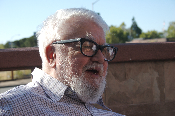
\includegraphics{McCarthy.png}
	\end{center}
	\caption{Fig. \ref{fig:mccarthy} -- John McCarthy}
	\label{fig:mccarthy}
\end{figure}

\href{https://fr.wikipedia.org/wiki/John_McCarthy}{John McCarthy}
\emph{(1927-2011)} auteur du langage
\href{https://fr.wikipedia.org/wiki/Lisp}{Lisp} en 1958, dont la
principale construction est la définition de \textbf{fonctions}. Il joua
un rôle majeur dans la programmation en intelligence artificielle,
écrivant un des premiers programmes jouant aux échecs.

    \hypertarget{notion-de-fonction-premiuxe8re-approche}{%
\section{Notion de fonction: première
approche}\label{notion-de-fonction-premiuxe8re-approche}}

Supposons que l'on doive afficher les valeurs des puissances de 2 les
plus utilisées en architecture machine (8, 16, 32 et 64). On peut
utiliser le programme du chapitre précédent:

    \begin{Verbatim}[commandchars=\\\{\}]
\PY{n}{N} \PY{o}{=} \PY{l+m+mi}{8}
\PY{n}{p} \PY{o}{=} \PY{l+m+mi}{1}
\PY{k}{for} \PY{n}{c} \PY{o+ow}{in} \PY{n+nb}{range}\PY{p}{(}\PY{n}{N}\PY{p}{)}\PY{p}{:}
    \PY{n}{p} \PY{o}{=} \PY{n}{p} \PY{o}{*} \PY{l+m+mi}{2}
\PY{n+nb}{print}\PY{p}{(}\PY{n}{p}\PY{p}{)}
\PY{n}{N} \PY{o}{=} \PY{l+m+mi}{16}
\PY{n}{p} \PY{o}{=} \PY{l+m+mi}{1}
\PY{k}{for} \PY{n}{c} \PY{o+ow}{in} \PY{n+nb}{range}\PY{p}{(}\PY{n}{N}\PY{p}{)}\PY{p}{:}
    \PY{n}{p} \PY{o}{=} \PY{n}{p} \PY{o}{*} \PY{l+m+mi}{2}
\PY{n+nb}{print}\PY{p}{(}\PY{n}{p}\PY{p}{)}
\PY{n}{N} \PY{o}{=} \PY{l+m+mi}{32}
\PY{n}{p} \PY{o}{=} \PY{l+m+mi}{1}
\PY{k}{for} \PY{n}{c} \PY{o+ow}{in} \PY{n+nb}{range}\PY{p}{(}\PY{n}{N}\PY{p}{)}\PY{p}{:}
    \PY{n}{p} \PY{o}{=} \PY{n}{p} \PY{o}{*} \PY{l+m+mi}{2}
\PY{n+nb}{print}\PY{p}{(}\PY{n}{p}\PY{p}{)}
\PY{n}{N} \PY{o}{=} \PY{l+m+mi}{64}
\PY{n}{p} \PY{o}{=} \PY{l+m+mi}{1}
\PY{k}{for} \PY{n}{c} \PY{o+ow}{in} \PY{n+nb}{range}\PY{p}{(}\PY{n}{N}\PY{p}{)}\PY{p}{:}
    \PY{n}{p} \PY{o}{=} \PY{n}{p} \PY{o}{*} \PY{l+m+mi}{2}
\PY{n+nb}{print}\PY{p}{(}\PY{n}{p}\PY{p}{)}
\end{Verbatim}

    Procéder de cette façon met en évidence plusieurs problèmes. On peut
citer:
\begin{itemize}
\item les répétitions; 
\item la difficulté de maintenance du code \emph{(que
devrait-on faire si on souhaite ensuite les puissances de 16?)} 
\end{itemize}
La solution consiste à isoler la partie de code qui se répète, lui
donner un nom et l'appeler lorsque c'est nécessaire.

 \hypertarget{passer-des-arguments}{%
\section{Passer des arguments et récupérer une valeur}\label{passer-des-arguments}}
Le langage python (\emph{comme les autres langages}) possède une construction permettant de résoudre leproblème précédent: la \textbf{définition de fonction}.

\begin{Shaded}
\begin{Highlighting}[]
\KeywordTok{def}\NormalTok{ nom_fonction(paramètre(s)):}
\NormalTok{    bloc_instructions}
\end{Highlighting}
\end{Shaded}

Le nom de la fonction doit \textbf{commencer par une lettre}, ne doit \textbf{pas être un
mot reservé} et doit être autant que possible explicite. Le bloc
d'instructions, qui constitue le corps de la fonction, \textbf{DOIT}
être indenté. La fonction peut avoir 0, 1 ou plus de paramètres. \par Créons
une première version d'une fonction destinée à afficher les puissances
de 2.

    \begin{Verbatim}[commandchars=\\\{\}]
\PY{k}{def} \PY{n+nf}{puissance}\PY{p}{(}\PY{n}{n}\PY{p}{)}\PY{p}{:}
    \PY{n}{p} \PY{o}{=} \PY{l+m+mi}{1}
    \PY{k}{for} \PY{n}{c} \PY{o+ow}{in} \PY{n+nb}{range}\PY{p}{(}\PY{n}{n}\PY{p}{)}\PY{p}{:}
        \PY{n}{p} \PY{o}{=} \PY{n}{p} \PY{o}{*} \PY{l+m+mi}{2}
    \PY{n+nb}{print}\PY{p}{(}\PY{n}{p}\PY{p}{)}
\end{Verbatim}

    Lorsqu'on exécute ce code, il ne se passe \textbf{rien}. \`A ce stade on a
définit la fonction, il faut maintenant l'appeler pour que tout son code
soit exécuté. L'appel d'une fonction consiste à écrire \textbf{son nom
suivi de parenthèses ouvrantes-fermantes} à l'intérieur desquelles on
place d'éventuels \textbf{arguments}.

    \begin{Verbatim}[commandchars=\\\{\}]
\PY{n}{puissance}\PY{p}{(}\PY{l+m+mi}{8}\PY{p}{)}
\PY{n}{puissance}\PY{p}{(}\PY{l+m+mi}{16}\PY{p}{)}
\PY{n}{puissance}\PY{p}{(}\PY{l+m+mi}{32}\PY{p}{)}
\PY{n}{puissance}\PY{p}{(}\PY{l+m+mi}{64}\PY{p}{)}
\end{Verbatim}

    La définition \texttt{puissance(n)} proposée ne correspond pas
exactement à une fonction (on devrait plutôt parler ici de
\emph{procédure}). En effet, une fonction au sens strict devrait fournir
(on dit \textbf{retourner}) une valeur. Python dispose de l'instruction
\texttt{return} qui permet de retourner une valeur. Une version
améliorée de la définition de \texttt{puissance(n)} ainsi que son appel
pourrait être:

    \begin{Verbatim}[commandchars=\\\{\}]
\PY{k}{def} \PY{n+nf}{puissance}\PY{p}{(}\PY{n}{n}\PY{p}{)}\PY{p}{:}
    \PY{n}{p} \PY{o}{=} \PY{l+m+mi}{1}
    \PY{k}{for} \PY{n}{c} \PY{o+ow}{in} \PY{n+nb}{range}\PY{p}{(}\PY{n}{n}\PY{p}{)}\PY{p}{:}
        \PY{n}{p} \PY{o}{=} \PY{n}{p} \PY{o}{*} \PY{l+m+mi}{2}
    \PY{k}{return} \PY{n}{p}

\PY{n+nb}{print}\PY{p}{(}\PY{n}{puissance}\PY{p}{(}\PY{l+m+mi}{8}\PY{p}{)}\PY{p}{)}
\PY{n+nb}{print}\PY{p}{(}\PY{n}{puissance}\PY{p}{(}\PY{l+m+mi}{16}\PY{p}{)}\PY{p}{)}
\PY{n+nb}{print}\PY{p}{(}\PY{n}{puissance}\PY{p}{(}\PY{l+m+mi}{32}\PY{p}{)}\PY{p}{)}
\PY{n+nb}{print}\PY{p}{(}\PY{n}{puissance}\PY{p}{(}\PY{l+m+mi}{64}\PY{p}{)}\PY{p}{)}
\end{Verbatim}

    \hypertarget{concevoir-une-fonction}{%
\section{Concevoir une fonction}\label{concevoir-une-fonction}}

En plus d'un nom explicite une fonction devrait être convenablement
documentée. Cette documentation devra comporter des
\textbf{spécifications}, c'est-à-dire les hypothèses faites sur les
arguments, leur relation avec le résultat retourné. On reviendra plus en détails sur cette notion de spécifications dans le cours d'algorithmique.\par En python, la
documentation suit immédiatement la définition de la fonction et est
encadrée de trois double quotes """. Cette partie constitue la \textbf{docstring}. \par
\newpage
Exemple
    \begin{Verbatim}[commandchars=\\\{\}]
\PY{k}{def} \PY{n+nf}{puissance}\PY{p}{(}\PY{n}{x}\PY{p}{,}\PY{n}{n}\PY{p}{)}\PY{p}{:}
    \PY{l+s+sd}{\PYZdq{}\PYZdq{}\PYZdq{}}
\PY{l+s+sd}{    Calcule x à la puissance n; on suppose x \PYZgt{} 0 et n \PYZgt{}= 0}
\PY{l+s+sd}{    \PYZdq{}\PYZdq{}\PYZdq{}}
    \PY{n}{p} \PY{o}{=} \PY{l+m+mi}{1}
    \PY{k}{for} \PY{n}{c} \PY{o+ow}{in} \PY{n+nb}{range}\PY{p}{(}\PY{n}{n}\PY{p}{)}\PY{p}{:}
        \PY{n}{p} \PY{o}{=} \PY{n}{p} \PY{o}{*} \PY{n}{x}
    \PY{k}{return} \PY{n}{p}

\PY{n+nb}{print}\PY{p}{(}\PY{n}{puissance}\PY{p}{(}\PY{l+m+mi}{16}\PY{p}{,}\PY{l+m+mi}{2}\PY{p}{)}\PY{p}{)}
\end{Verbatim}

    \begin{Verbatim}[commandchars=\\\{\}]
256
    \end{Verbatim}

    Cette documentation est en outre accessible via la fonction
\texttt{help()}

    \begin{Verbatim}[commandchars=\\\{\}]
\PY{n}{help}\PY{p}{(}\PY{n}{puissance}\PY{p}{)}
\end{Verbatim}

    \begin{Verbatim}[commandchars=\\\{\}]
Help on function puissance in module \_\_main\_\_:
puissance(x, n)
    Calcule x à la puissance n; on suppose x > 0 et n >= 0
    \end{Verbatim}

    \hypertarget{fonctions-de-la-bibliothuxe8que-standard}{%
\section{Fonctions de la bibliothèque
standard}\label{fonctions-de-la-bibliothuxe8que-standard}}

Tous les grands langages de programmation proposent des fonctions toutes
faites. Ces fonctions écrites dans le langage et fournies avec lui sont
regroupées dans la \textbf{bibliothèque standard}. Dans la bibliothèque standard de python on trouve par
exemple, la bibliothèque \emph{math} ou \emph{random}. Pour pouvoir
utiliser les fonctions d'une bibliothèque, il faut d'abord l'importer
avec l'instruction \texttt{import}.
    \begin{Verbatim}[commandchars=\\\{\}]
\PY{k+kn}{import} \PY{n+nn}{math}
\end{Verbatim}

    Pour obtenir la documentation d'une fonction de la bibliothèque (on dit
aussi \emph{module}), on utilise la fonction \texttt{help()}.

    \begin{Verbatim}[commandchars=\\\{\}]
\PY{n}{help}\PY{p}{(}\PY{n}{math}\PY{o}{.}\PY{n}{radians}\PY{p}{)}
\end{Verbatim}

    Pour connaître les fonctions disponibles dans une bibliothèque, on
utilise la fonction \texttt{dir()}.

    \begin{Verbatim}[commandchars=\\\{\}]
\PY{n+nb}{dir}\PY{p}{(}\PY{n}{math}\PY{p}{)}
\end{Verbatim}
    Pour appeler une fonction d'une bibliothèque, on doit préfixer son nom
par le \textbf{nom de la bibliothèque suivi d'un point}.
    \begin{Verbatim}[commandchars=\\\{\}]
\PY{k+kn}{import} \PY{n+nn}{math}
\PY{c+c1}{\PYZsh{}Affichage du sinus de pi/4}
\PY{n+nb}{print}\PY{p}{(}\PY{l+s+s2}{\PYZdq{}}\PY{l+s+s2}{Sinus de pi/4: }\PY{l+s+s2}{\PYZdq{}}\PY{p}{,} \PY{n}{math}\PY{o}{.}\PY{n}{sin}\PY{p}{(}\PY{n}{math}\PY{o}{.}\PY{n}{pi}\PY{o}{/}\PY{l+m+mi}{4}\PY{p}{)}\PY{p}{)}
\end{Verbatim}

    \begin{Verbatim}[commandchars=\\\{\}]
Sinus de pi/4:  0.7071067811865476

    \end{Verbatim}

    On peut raccourcir l'écriture précédente, même si ce n'est pas
très recommandable, avec la construction suivante:

    \begin{Verbatim}[commandchars=\\\{\}]
\PY{k+kn}{from} \PY{n+nn}{math} \PY{k}{import} \PY{o}{*}

\PY{n+nb}{print}\PY{p}{(}\PY{l+s+s2}{\PYZdq{}}\PY{l+s+s2}{Sinus de pi/4:}\PY{l+s+s2}{\PYZdq{}}\PY{p}{,} \PY{n}{sin}\PY{p}{(}\PY{n}{pi}\PY{o}{/}\PY{l+m+mi}{4}\PY{p}{)}\PY{p}{)}
\end{Verbatim}
    \hypertarget{a-retenir}{%
\subsection{\`A retenir}\label{a-retenir}}

Une fonction permet une écriture plus concise du code, une maintenance
plus aisée. On la déclare de la manière suivante:

\begin{Shaded}
\begin{Highlighting}[]
\KeywordTok{def}\NormalTok{ nom_fonction(paramètre(s)):}
\NormalTok{    bloc_instructions}
\end{Highlighting}
\end{Shaded}

L'appel se fait en écrivant le nom de la fonction suivi d'éventuels
arguments entre parenthèses. Si la fonction ne retourne pas de valeur on
lui préfèrera le nom de \emph{procédure}. La bibliothèque standard
contient des fonctions prêtes à l'emploi. L'appel se fait de la même
manière, après l'importation de la bibliothèque avec l'instruction
\texttt{import}.

    \begin{center}\rule{0.5\linewidth}{\linethickness}\end{center}

\noindent\textbf{E1C2 : maximum}\\
Définissez une fonction maximum(\(n_1,n_2,n_3\)) qui renvoie le plus
grand de 3 nombres \(n_1, n_2, n_3\) fournis en arguments. Par exemple,
l'exécution de l'instruction :
\begin{Shaded}
\begin{Highlighting}[]
\BuiltInTok{print}\NormalTok{(maximum(}\DecValTok{2}\NormalTok{,}\DecValTok{5}\NormalTok{,}\DecValTok{4}\NormalTok{))}
\end{Highlighting}
\end{Shaded}
doit donner le résultat 5.

\noindent\textbf{E2C2 : volume d'un ballon}
\begin{enumerate}
\item \'Ecrire une fonction \texttt{volume\_ballon} qui prend en paramètre un rayon \(r\)
et qui retourne le volume \(V\) d'un ballon de rayon \(r\). Rappel:
\(V=\dfrac{4}{3}\times\pi r^{3}\)
\item Documenter la fonction. Afficher le volume d'un ballon de football
(\(r=11\) cm) puis de basket (\(r=12.4\) cm) en arrondissant les
résultats (voir la fonction \texttt{round()}de la bibliothèque
standard).
\end{enumerate}
\textbf{E3C2 : longueur d'un tweet}\par
La longueur maximale d'un message sur Tweeter est de 280 caractères. On
souhaite écrire un programme qui indique le nombre de caractères d'un
message qu'on souhaiterait publier.
\begin{enumerate}
\item Que réalise la fonction \texttt{len()} de la bibliothèque standard?
\item \'Ecrire une fonction longueur\_message(msg) qui prend comme paramètre
un message (\emph{une chaine de caractère}) et qui renvoit le nombre de
caractères de ce message. 
\item \'Ecrire le programme qui demande à
l'utilisateur de rentrer son message et qui affiche la longueur de
celui-ci. Utiliser la fonction précédente.
\end{enumerate}
\textbf{P1C2 : distance euclidienne}
(\href{http://www.france-ioi.org/}{France IOI})\\
Sur les feuilles à motifs que vous leur avez imprimées tout à l'heure,
les jeunes gens souhaiteraient calculer la distance entre deux motifs,
ce qui ce fait facilement si l'on perçoit la feuille comme un repère
orthonormé. Ce que doit faire votre programme :

Écrivez une fonction qui prend en paramètre les coordonnées
\((x_A,y_A)\) et \((x_B,y_B)\) de deux points et retourne la distance
euclidienne entre ces deux points. On rappelle que la distance
euclidienne entre deux points est égale à :
\[\sqrt{(x_B−x_A)^2+(y_B−y_A)^2}\]

Utilisez ensuite cette fonction dans un programme qui lit quatre nombres
décimaux \(x_A, y_A, x_B\) et \(y_B\) tapés au clavier, puis affiche la
distance entre les deux points correspondants.

On pourra utiliser la fonction \(sqrt(x)\) de la bibliothèque math, qui
retourne la racine carrée du paramètre \(x\).

\vspace{3cm} 
 Ce(tte) œuvre est mise à disposition selon les termes de la Licence
\href{https://creativecommons.org/licenses/by-nc/4.0/}{Creative Commons Attribution - Pas d'Utilisation Commerciale 4.0
International.}
\begin{center}

\includegraphics{Cc-by-nc_icon.svg.png}
\end{center}      

\newpage
    \hypertarget{correction}{%
\section{CORRECTION}\label{correction}}

\hypertarget{e1c2-maximum}{%
\subsection{E1C2 : maximum}\label{e1c2-maximum}}

    \begin{Verbatim}[commandchars=\\\{\}]
\PY{k}{def} \PY{n+nf}{maximum}\PY{p}{(}\PY{n}{n1}\PY{p}{,}\PY{n}{n2}\PY{p}{,}\PY{n}{n3}\PY{p}{)}\PY{p}{:}
    \PY{n}{maxi} \PY{o}{=} \PY{n}{n1}
    \PY{k}{if} \PY{n}{n2} \PY{o}{\PYZgt{}} \PY{n}{n1}\PY{p}{:}
        \PY{k}{if} \PY{n}{n3} \PY{o}{\PYZgt{}} \PY{n}{n2}\PY{p}{:}
            \PY{n}{maxi} \PY{o}{=} \PY{n}{n3}
        \PY{k}{else}\PY{p}{:}
            \PY{n}{maxi} \PY{o}{=} \PY{n}{n2}
    \PY{k}{return} \PY{n}{maxi}

\PY{n+nb}{print}\PY{p}{(}\PY{n}{maximum}\PY{p}{(}\PY{l+m+mi}{12}\PY{p}{,}\PY{l+m+mi}{5}\PY{p}{,}\PY{l+m+mi}{4}\PY{p}{)}\PY{p}{)}
\end{Verbatim}

    \hypertarget{e2c2-volume-dun-ballon}{%
\subsection{E2C2 : volume d'un ballon}\label{e2c2-volume-dun-ballon}}

    \begin{Verbatim}[commandchars=\\\{\}]
\PY{n}{help}\PY{p}{(}\PY{n+nb}{pow}\PY{p}{)}
\PY{n}{help}\PY{p}{(}\PY{n+nb}{round}\PY{p}{)}
\end{Verbatim}

    \begin{Verbatim}[commandchars=\\\{\}]
\PY{k+kn}{import} \PY{n+nn}{math}
\PY{k}{def} \PY{n+nf}{volume\PYZus{}ballon}\PY{p}{(}\PY{n}{r}\PY{p}{)}\PY{p}{:}
    \PY{l+s+sd}{\PYZdq{}\PYZdq{}\PYZdq{}}
\PY{l+s+sd}{    Calcule le volume d\PYZsq{}une boule de rayon r;}
\PY{l+s+sd}{    On suppose r \PYZgt{} 0.}
\PY{l+s+sd}{    \PYZdq{}\PYZdq{}\PYZdq{}}
    \PY{n}{V} \PY{o}{=} \PY{p}{(}\PY{l+m+mi}{4}\PY{o}{/}\PY{l+m+mi}{3}\PY{p}{)} \PY{o}{*} \PY{n}{math}\PY{o}{.}\PY{n}{pi} \PY{o}{*} \PY{n}{r}\PY{o}{*}\PY{o}{*}\PY{l+m+mi}{3}
    \PY{c+c1}{\PYZsh{}la puissance se note ** en python}
    \PY{c+c1}{\PYZsh{}Autre solution: V = (4/3) * math.pi * pow(r,3)}
    \PY{c+c1}{\PYZsh{}Voir help(pow)}
    \PY{k}{return} \PY{n+nb}{round}\PY{p}{(}\PY{n}{V}\PY{p}{)}

\PY{n+nb}{print}\PY{p}{(}\PY{l+s+s2}{\PYZdq{}}\PY{l+s+s2}{Volume ballon foot: }\PY{l+s+s2}{\PYZdq{}}\PY{p}{,}\PY{n}{volume\PYZus{}ballon}\PY{p}{(}\PY{l+m+mi}{11}\PY{p}{)}\PY{p}{,}\PY{l+s+s2}{\PYZdq{}}\PY{l+s+s2}{cm3}\PY{l+s+s2}{\PYZdq{}}\PY{p}{)}
\PY{n+nb}{print}\PY{p}{(}\PY{l+s+s2}{\PYZdq{}}\PY{l+s+s2}{Volume ballon basket: }\PY{l+s+s2}{\PYZdq{}}\PY{p}{,}\PY{n}{volume\PYZus{}ballon}\PY{p}{(}\PY{l+m+mf}{12.4}\PY{p}{)}\PY{p}{,}\PY{l+s+s2}{\PYZdq{}}\PY{l+s+s2}{cm3}\PY{l+s+s2}{\PYZdq{}}\PY{p}{)}
\end{Verbatim}

    \hypertarget{e3c2-longueur-dun-tweet}{%
\subsection{E3C2 : longueur d'un tweet}\label{e3c2-longueur-dun-tweet}}

    \begin{Verbatim}[commandchars=\\\{\}]
\PY{n}{help}\PY{p}{(}\PY{n+nb}{len}\PY{p}{)}
\end{Verbatim}

    \begin{Verbatim}[commandchars=\\\{\}]
\PY{k}{def} \PY{n+nf}{longueur\PYZus{}message}\PY{p}{(}\PY{n}{msg}\PY{p}{)}\PY{p}{:}
    \PY{l+s+sd}{\PYZdq{}\PYZdq{}\PYZdq{}}
\PY{l+s+sd}{    Calcule la longueur d\PYZsq{}un message msg;}
\PY{l+s+sd}{    msg est une chaine de caractères.}
\PY{l+s+sd}{    \PYZdq{}\PYZdq{}\PYZdq{}}
    \PY{k}{return} \PY{n+nb}{len}\PY{p}{(}\PY{n}{msg}\PY{p}{)}

\PY{n}{tweet} \PY{o}{=} \PY{n+nb}{input}\PY{p}{(}\PY{l+s+s2}{\PYZdq{}}\PY{l+s+s2}{Quel message souhaitez\PYZhy{}vous publier? }\PY{l+s+s2}{\PYZdq{}}\PY{p}{)}
\PY{n}{l} \PY{o}{=} \PY{n}{longueur\PYZus{}message}\PY{p}{(}\PY{n}{tweet}\PY{p}{)}
\PY{n+nb}{print}\PY{p}{(}\PY{l+s+s2}{\PYZdq{}}\PY{l+s+s2}{Sa longueur est de}\PY{l+s+s2}{\PYZdq{}}\PY{p}{,} \PY{n}{l}\PY{p}{,} \PY{l+s+s2}{\PYZdq{}}\PY{l+s+s2}{caractères}\PY{l+s+s2}{\PYZdq{}}\PY{p}{)}
\end{Verbatim}

    \begin{Verbatim}[commandchars=\\\{\}]
Quel message souhaitez-vous publier? 
Sa longueur est de 0 caractères

    \end{Verbatim}

    \hypertarget{p1c2-distance-euclidienne}{%
\subsection{P1C2 : distance
euclidienne}\label{p1c2-distance-euclidienne}}

    \begin{Verbatim}[commandchars=\\\{\}]
\PY{k+kn}{import} \PY{n+nn}{math} 

\PY{k}{def} \PY{n+nf}{d\PYZus{}euclide}\PY{p}{(}\PY{n}{xA}\PY{p}{,}\PY{n}{xB}\PY{p}{,}\PY{n}{yA}\PY{p}{,}\PY{n}{yB}\PY{p}{)}\PY{p}{:}
    \PY{l+s+sd}{\PYZdq{}\PYZdq{}\PYZdq{}}
\PY{l+s+sd}{    Calcule la distance euclidienne entre deux points A et B de coordonnées }
\PY{l+s+sd}{    (xA,yA) et (xB,yB);}
\PY{l+s+sd}{    On suppose que xA,xB,yA,yB sont des flottants.}
\PY{l+s+sd}{    \PYZdq{}\PYZdq{}\PYZdq{}}
    \PY{n}{d2} \PY{o}{=} \PY{p}{(}\PY{n}{xB}\PY{o}{\PYZhy{}}\PY{n}{xA}\PY{p}{)}\PY{o}{*}\PY{o}{*}\PY{l+m+mi}{2} \PY{o}{+} \PY{p}{(}\PY{n}{yB}\PY{o}{\PYZhy{}}\PY{n}{yA}\PY{p}{)}\PY{o}{*}\PY{o}{*}\PY{l+m+mi}{2}
    \PY{k}{return} \PY{n}{math}\PY{o}{.}\PY{n}{sqrt}\PY{p}{(}\PY{n}{d2}\PY{p}{)}

\PY{n+nb}{print}\PY{p}{(}\PY{l+s+s2}{\PYZdq{}}\PY{l+s+s2}{\PYZhy{}\PYZhy{}\PYZhy{}\PYZhy{}\PYZhy{} Distance entre deux points A et B \PYZhy{}\PYZhy{}\PYZhy{}\PYZhy{}\PYZhy{}\PYZhy{}\PYZhy{}\PYZhy{}}\PY{l+s+s2}{\PYZdq{}}\PY{p}{)}
\PY{n+nb}{print}\PY{p}{(}\PY{l+s+s2}{\PYZdq{}}\PY{l+s+s2}{Entrez dans l}\PY{l+s+s2}{\PYZsq{}}\PY{l+s+s2}{ordre xA, yA, xB, yB }\PY{l+s+s2}{\PYZdq{}}\PY{p}{)}
\PY{n}{xA}\PY{p}{,} \PY{n}{xB}\PY{p}{,} \PY{n}{yA}\PY{p}{,} \PY{n}{yB} \PY{o}{=} \PY{n+nb}{float}\PY{p}{(}\PY{n+nb}{input}\PY{p}{(}\PY{p}{)}\PY{p}{)}\PY{p}{,} \PY{n+nb}{float}\PY{p}{(}\PY{n+nb}{input}\PY{p}{(}\PY{p}{)}\PY{p}{)}\PY{p}{,} \PY{n+nb}{float}\PY{p}{(}\PY{n+nb}{input}\PY{p}{(}\PY{p}{)}\PY{p}{)}\PY{p}{,} \PY{n+nb}{float}\PY{p}{(}\PY{n+nb}{input}\PY{p}{(}\PY{p}{)}\PY{p}{)}
\PY{n+nb}{print}\PY{p}{(}\PY{l+s+s2}{\PYZdq{}}\PY{l+s+s2}{La distance entre A et B est}\PY{l+s+s2}{\PYZdq{}}\PY{p}{,} \PY{n}{d\PYZus{}euclide}\PY{p}{(}\PY{n}{xA}\PY{p}{,}\PY{n}{xB}\PY{p}{,}\PY{n}{yA}\PY{p}{,}\PY{n}{yB}\PY{p}{)}\PY{p}{)}
\end{Verbatim}


    % Add a bibliography block to the postdoc
    
    
    
    \end{document}
